% -----------------------------------------------
% Template for ISMIR Papers
% 2020 version, based on previous ISMIR templates

% Requirements :
% * 6+n page length maximum
% * 4MB maximum file size
% * Copyright note must appear in the bottom left corner of first page
% * Clearer statement about citing own work in anonymized submission
% (see conference website for additional details)
% -----------------------------------------------

\documentclass{article}
\usepackage[T1]{fontenc} % add special characters (e.g., umlaute)
\usepackage[utf8]{inputenc} % set utf-8 as default input encoding
\usepackage{ismir,amsmath,cite,url}
\usepackage{graphicx}
\usepackage{color}

% Optional: To use hyperref, uncomment the following.
% \usepackage[bookmarks=false,hidelinks]{hyperref}
% Mind the bookmarks=false option; bookmarks are incompatible with ismir.sty.

\usepackage{lineno}
\linenumbers

% Title.
% ------
\title{Neural models for computer-assisted musical orchestration: a preliminary study}

% Note: Please do NOT use \thanks or a \footnote in any of the author markup

% Single address
% To use with only one author or several with the same address
% ---------------
%\oneauthor
% {Names should be omitted for double-blind reviewing}
% {Affiliations should be omitted for double-blind reviewing}

% Two addresses
% --------------
%\twoauthors
%  {First author} {School \\ Department}
%  {Second author} {Company \\ Address}

%% To make customize author list in Creative Common license, uncomment and customize the next line
%  \def\authorname{First Author, Second Author}


% Three addresses
% --------------
\threeauthors
  {First Author} {Affiliation1 \\ {\tt author1@ismir.edu}}
  {Second Author} {\bf Retain these fake authors in\\\bf submission to preserve the formatting}
  {Third Author} {Affiliation3 \\ {\tt author3@ismir.edu}}

%% To make customize author list in Creative Common license, uncomment and customize the next line
%  \def\authorname{First Author, Second Author, Third Author}

% Four or more addresses
% OR alternative format for large number of co-authors
% ------------
%\multauthor
%{First author$^1$ \hspace{1cm} Second author$^1$ \hspace{1cm} Third author$^2$} { \bfseries{Fourth author$^3$ \hspace{1cm} Fifth author$^2$ \hspace{1cm} Sixth author$^1$}\\
%  $^1$ Department of Computer Science, University , Country\\
%$^2$ International Laboratories, City, Country\\
%$^3$  Company, Address\\
%{\tt\small CorrespondenceAuthor@ismir.edu, PossibleOtherAuthor@ismir.edu}
%}
%\def\authorname{First author, Second author, Third author, Fourth author, Fifth author, Sixth author}


\sloppy % please retain sloppy command for improved formatting

\begin{document}

%
\maketitle
%
\begin{abstract}
In this paper we will explore preliminary neural models for the task of computer-assisted musical orchestration. After an introduction on the problem, we will show how we decided to model musical orchestration as a classification task. In this context, we will propose two deep learning models and we will show how they perform as classifiers for musical instruments recognition by comparing them with specific baselines. We will the show how they perform, both qualitative and quantitative, in the task of computer-assisted orchestration by comparing them with state-of-the-art systems. We will highlight, finally, benefits and problems of neural approaches for orchestration and we will propose possible future steps.
\end{abstract}
%
\section{Introduction}\label{sec:introduction}

\section{Data generation}

\subsection{Sources}
We used the TinySOL database to create our input data. This database contains samples of notes played using the ordinario style and with three different dynamics for each pair of instrument and pitch : \textit{pp}, \textit{mf} and \textit{ff}. The exact list of samples is shown in Tab.\ref{tab_pitch}.  \textbf{(Should we talk more about TinySOL here?)}

Since the goal was to train the model to detect multiple instruments playing simultaneously, the samples used for training were generated by mixing a random combination of instruments and pitches. More precisely, given the number $N$ of instruments playing at the same time, the data was generated as follows:

\begin{itemize}
\item An orchestra of $N$ instruments is chosen in advance (it is the same for all samples).
\item For each instrument in the orchestra, a random note is picked among the corresponding available samples in TinySOL.
\item For each chosen note, a random dynamic is picked.
\item The samples are added and normalized by the number of instruments.
\item The Mel spectrogram of the mixture is then computed and used as input of the model.
\end{itemize}

The choice of Mel spectrograms as input features of the model is very commmon in music information \textbf{\{Insert reference\}} and can be considered to be an accurate representation of the way humans perceive sound and music.\\

Samples had a sample rate of $44100Hz$ and were all padded or chopped to be exactly 4 seconds long. The Mel spectrograms were then generated using an FFT hop length of 2048 samples (e.g. the window of each FFT was $46ms$ wide), and a number of Mel bins equal to 128. Therefore, all the features fed to the model were matrices of size $128\times 345$. We used Librosa package in Python to compute the features, and more details on the exact computations can be found in \textbf{\{Reference to Librosa\}} The choice of the hop length was made by doing a compromise between the amount of information extracted by each FFT window, and the ability to capture changes in the dynamic, assuming that no change faster than $10ms$ could be perceived by the human ear.

\begin{table}
\begin{tabular}{|c|c|c|}
\hline
Instrument & Abbreviation & Range \\
\hline
Violin & Vn & G3-E7\\
Cello & Vc & C2-C6\\
Viola & Va & C3-C7\\
Trumpet C & TpC & F\#3-C6\\
Trombone & Tbn & A\#0;A\#1-C5\\
Oboe & Ob & A\#3-A6\\
Horn & Hn & G1-F5\\
Flute & Fl & B3-D7\\
Clarinette Bb & ClBb & D3-G6\\
Contrabass & Cb & E1-C5\\
Bass Tuba & BTb & F\#1-F4\\
Bassoon & Bn & A\#1-D\#5\\
\hline
\end{tabular}
\begin{caption}Table containing the pitch ranges in the TinySOL database, used for training. Hyphen means all the notes between the two explicited notes. \label{tab_pitch}
\end{caption}
\end{table}

\subsection{Data augmentation}

In order to increase the variability of the samples, we used two methods of data augmentation on the samples.\\

The first one was done on the mixture of the samples, by slightly shifting the frequency of the signal. In practice, the sample rate used to compute the Mel spectrogram was modified to be within $5\%$ of the acual $44100Hz$.\\

The second one was done on the Mel spectrogram, by setting to 0 random columns and rows of the feature matrices. For a given matrix, each column and each row had individually a $1\%$ chance to be set to 0, which yielded an average of $1.28$ reset columns and $3.45$ reset rows. This method of data augmentation aimed to be more resilient to the possible errors of recording, due either to a setup that induces interferences and cancels specific frequences, or to a default in the microphone that fails to record a small temporal portion.

\section{Our model}
- deep learning trained for classification and then used for orchestraion
- changing number of instruments

Our idea is to perform orchestration using deep neural networks trained for classification. By generating input data that is combinations of different instruments and pitches, the network learns how to take a sound that is a complex combination of notes and timbres and deconstruct it into its original parts. Then, when a network is given a target sound as input, it will attempt to apply the same classification rules, outputing a vector of the probabilities of each sample being in the target sound. By taking the samples that have the highest probability, an orchestrated solution can be created. 

We did not train our model to classify the dynamics of a sample despite TinySOL having pianissimo, mezzo forte, and fortissimo recordings for each sample. If we had, then each class would have only one data point. Instead, when the model is used for orchestration, the dynamic is determined by the probability of that sample as output by the model. If the model output a probability higher than $0.66$ for a sample, the fortissimo version of the sample was used. If it was between $0.33$ and $0.66$, then the mezzo forte version, and if less than $0.33$ the pianissimo dynamic. \textbf{\{I am not sure this hypothesis can be used accurately\}}

\subsection{Baseline}
In order to have a baseline to compare our results against, we attempted to solve the classification problem using various parametric classifiers. The classifiers we tested were Support Vector Machine (SVM), Random Forest, and K-Nearest Neighbors. We used the implementations provided in the scikit-learn library for each classifier. For SVM, we used SVC with an RBF kernel. For Random Forest, we set the maximum depth of each tree to be 15. Each classifier was wrapped in a MultiOutputClassifier to achieve the multi-label nature of this problem. We found SVM to have the highest accuracy of the three classifiers across all experiments. All of the following baselin experiments used 50,000 generated samples with a train-test split of 60/40. Each sample is a combination of one or more instruments and is four seconds in length. The features used are the mel frequency cepstral coefficients (MFCCs) of the resulting combination, with a total of 100 coefficients per sample.

We started by simplifying the problem to classifying only the instruments and not the pitch. This had the benefit of both reducing the number of classes and increasing the number of samples per class. We found that SVM was able to very accurately identify the instrument given an input that had only one instrument present; for this case the accuracy was 99.8\%. However as soon as multiple instruments were present in the input, the accuracy dropped significantly. With two instruments, accuracy was 55.4\%, with three it was 19.6\% and with 10 instruments the accuracy was 0.5\%. 

To better approximate the problem of identifying instrument and pitch, we then attempted to classify the instrument and pitch class. That is, which octave the pitch was in did not matter, only the pitch class. The input was a combination of two instruments drawn from a possible twelve instruments, and the classifier attempted to identify which instruments were present and for two of those instruments, say Flute and Violin, which pitch classes were present. If another instrument was present that was not Flute or Violin, the classifier would attempt to identify that instrument, but not its pitch class. The best results from this setting of the problem was SVM with 30.2\% accuracy, which was a result of classifying the pitch class of Flute and Violin. Depending on which two instruments had their pitch class identified, the accuracy varied greatly. For a Violin and Cello accuracy was 20.9\%, and for Trombone and Bass Tuba accuracy was 2.2\%.

For a slight modification on this setting, we no longer attempted to identify which instrument was present if it was not one of the two instruments whose pitch class was being identified. Instead, the classifier would simply identify that an instrument that was not one of the two was present. Since this is a simpler problem, it lead to increased accuracies. The accuracies from this experiment are outlined in Table 1. Since Random Forest performed worse than SVM is every experiment, we stopped testing with Random Forest and used SVM from that point on.

We then performed this same experiment with three instruments having their pitch class identified. Each input was a combination of three instruments drawn from a possible twelve instruments. For three instruments specified in that experiment, pitch class was identified. Flute, Oboe, and Violin reached an accuracy of 11.1\%, and Bass Tuba, Trumpet, and Trombone was 0.5\%. As we increased the number of instruments whose pitch classes was being identified, the accuracy continued to drop. For classifying the pitch class of four instruments: Oboe, French Horn, Violin, and Flute, the accuracy was 2.7\%.

This was still a simplified version of the problem, as we were identifying only the pitch class of a few instruments. However, the parametric classifiers were unable to achieve accurate results as the number of instruments increased. Therefore, we did not attempt the full setting of the problem, in which individual pitches are classified for all instruments, with parametric classifiers. 

\begin{table}
  \begin{center}
    \label{tab:table1}
    \begin{tabular}{c|c|c|c} 
    	  \hline
      \textbf{Instr. 1} & \textbf{Instr. 2} & \textbf{SVM Accuracy} & \textbf{RF Accuracy}\\
      \hline
      Violin & Flute & 38.8\% & 9.8\% \\
      \hline
      Violin & Trumpet & 33.8\% & 9.1\% \\
      \hline
      Violin & Cello & 34.8\% & 6.3\% \\
      \hline
      Cello & Viola & 32.1\% & 5.8\% \\
      \hline
      Oboe & French Horn & \textbf{39.9\%} & \textbf{17.5\%} \\
      \hline
    \end{tabular}
  \end{center}
  \caption{Comparison of results between SVM and Random Forest. Each data point is a combination of two TinySOL samples, where at least one of the samples is from one of the two instruments specified for that experiment. For the samples drawn from one of the two instruments, the pitch class of that sample is identified. For a sample not from one of the two instruments, the classifier simply attempted to identify that a sample from one of the non-specified instruments was present. In this setting, there are 25 classes: 24 from the 12 pitch classes from 2 instruments, and 1 class that specified whether an instrument that is not one of the two specified is present.}
\end{table}


\subsection{CNN with LSTM}

The first deep model we tested was a Convolutional Neural Network (CNN). CNN shows good performance on classification assignment for its strong ability to extract spacial features, so we implemented a basic CNN with three convolutional layers and two fully connected layers. Each convolutional layer is followed by a BatchNorm layer, a ReLU activation layer and a 2 * 2  MaxPool layer with a stride of 2. The kernel size is 3 * 3 with a stride of 1 and a padding of 1. The number of filters are 8, 16, 32. This setting is simple but we can make a good comparison between it and the baseline. \\

\begin{figure}
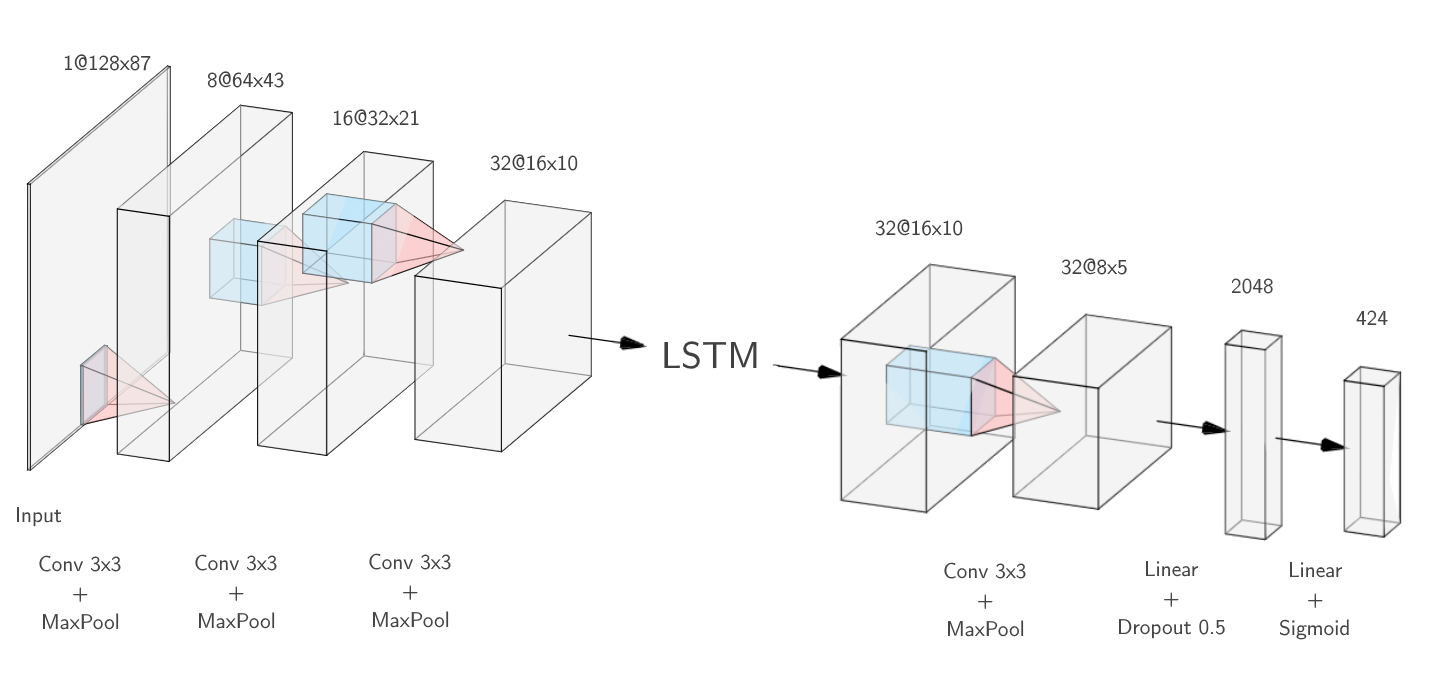
\includegraphics[scale=0.45]{CNN_LSTM_diagram.png}
\caption{Diagram of the CNN with LSTM architecture. \label{cnn_lstm}}
\end{figure}

Given that audio is one kind of sequential data, it is easy to consider Long Short-Term Memory network(LSTM) as test model. In our setting, we added one LSTM layer with 32 outputs units following three convolutional layers following the same pattern as the CNN described earlier. After LSTM layer, we reshaped the output into the same size as the output of the last convulational layer, which was fed to another convolutional layer with the same structure and kernel size, yielding a tensor of dimensions $32\times 8 \times 21$. Finally, we flattened out the outputs and fed them into fully a connected layer with Dropout layer, followed by another fully connected layer. Finally, the sigmoid function was applied to th final layer in order to get a probability between 0 and 1 for each individual label.\\


\subsection{ResNet}

The second deep model that we used was the well known deep residual network ResNet.

To make our setting more reasonable, we took the well-known deep residual network(ResNet) as backbone in our experiments. Specifically, we used 18-layer ResNet. Besides, to make the model more suitable to our problem, we reset the output channel numbers of each block with 32, 64, 32, 32 respectively. 

\subsection{Classification results}

During training, the loss function used to optimize the inner parameters of the model was binary cross entropy, as it is the common choice for multiclass multilabel classification frameworks such as this one. However, the value of the loss function alone is difficult to interpret. This is why, we used a complementary function $f$ only for evaluation, to match the notion of accuracy of the model with the intuitive approach. This function compares a vector of expected outputs $\overline{X}$ with the estimated output from the model $\hat{X}$ by using the following function

\begin{equation}
f(\overline{X}, \hat{X}) = \frac{1}{N}<\overline{X}, M_N(\hat{X})>
\label{eval}
\end{equation}

where

\begin{equation}
M_N(\hat{X})_i = \left\{\begin{array}{ll}
1 \text{ if } i \in I_N(\hat{X})\\
0 \text{ otherwise}
\end{array}\right.
\label{NMax}
\end{equation}
and $I_N(\hat{X})$ is the set of the indices containing the $N$ first maximums of the vector $\hat{X}$.\\

More specifically, the function $M_N(\hat{X})$ takes as an input a vector of probabilities (values between 0 and 1) and outputs a vector where only the positions of the $N$ first maxima are set to 1. This new vector would be the orchestration of $N$ instruments given by the model. Thus, the function $f$ simply outputs the proportion of the estimated orchestration that matches the expected one.\\

Different experiments were made by varying the number of instruments in the orchestra $N$ but always matching this number with the number of instruments in each mixture sample. Tab. \ref{exp_tab} shows the orchestra for each different value of $N$ used in the experiments.\\

\begin{table}
\begin{tabular}{|c|l|}
\hline
$N$ & Orchestra\\
\hline
4 & Hn, Ob, Vn, Va\\
5 & Hn, Ob, Vn, Va, Vc\\
6 & Hn, Ob, Vn, Va, Vc, Fl\\
7 & Hn, Ob, Vn, Va, Vc, Fl, Tbn\\
8 & Hn, Ob, Vn, Va, Vc, Fl, Tbn, Bn\\
9 & Hn, Ob, Vn, Va, Vc, Fl, Tbn, Bn, TpC\\
10 & Hn, Ob, Vn, Va, Vc, Fl, Tbn, Bn, TpC, ClBb\\
\hline
\end{tabular}

\begin{caption}
Orchestra for each $N$ used in the experiments.
\label{exp_tab}
\end{caption}
\end{table}

Then, for both CNN with LSTM and ResNet, we computed the maximum accuracy over the epochs. Tab. \ref{epoch} compiles the number of samples per epoch and the total number of epochs used for each model and each value of $N$. Tab. \ref{class_res} shows the maximum accuracy computed using the function $f$ explicited in (\ref{eval}).



\begin{table}
\begin{tabular}{|c|c|c|c|}
\hline
Model & $N$ & Nb epochs & Nb samples\\
\hline
CNN-LSTM & 4-7 & 50 & 100000 \\
CNN-LSTM & 8-10 & 50 & 200000 \\
ResNet & 4-8 & 20 & 200000 \\
ResNet & 9-10 & 20 & 400000 \\
\hline
\end{tabular}

\begin{caption}
Number of epochs and number of samples per epoch used for training each model with a given value of the size of the orchestra $N$.
\label{epoch}
\end{caption}
\end{table}


\begin{table}
\begin{tabular}{|c|c|c|c|c|c|c|c|c|c|c|c|c|c|c|}
\hline
Instruments & \multicolumn{2}{c|}{$N=4$} & \multicolumn{2}{c|}{$N=5$}& \multicolumn{2}{c|}{$N=6$}& \multicolumn{2}{c|}{$N=7$}& \multicolumn{2}{c|}{$N=8$}& \multicolumn{2}{c|}{$N=9$}& \multicolumn{2}{c|}{$N=10$}\\
\cline{2-3} & C & R & C & R & C & R & C & R & C & R & C & R & C & R\\
\hline
All & 0 & 0 & 0 & 0 & 0 & 0 & 0 & 0 & 0 & 0 & 0 & 0 & 0 & 0\\
Hn & 0 & 0 & 0 & 0 & 0 & 0 & 0 & 0 & 0 & 0 & 0 & 0 & 0 & 0\\
Ob & 0 & 0 & 0 & 0 & 0 & 0 & 0 & 0 & 0 & 0 & 0 & 0 & 0 & 0\\
Vn & 0 & 0 & 0 & 0 & 0 & 0 & 0 & 0 & 0 & 0 & 0 & 0 & 0 & 0\\
Va & 0 & 0 & 0 & 0 & 0 & 0 & 0 & 0 & 0 & 0 & 0 & 0 & 0 & 0\\
Vc & 0 & 0 & 0 & 0 & 0 & 0 & 0 & 0 & 0 & 0 & 0 & 0 & 0 & 0\\
Fl & 0 & 0 & 0 & 0 & 0 & 0 & 0 & 0 & 0 & 0 & 0 & 0 & 0 & 0\\
Tbn & 0 & 0 & 0 & 0 & 0 & 0 & 0 & 0 & 0 & 0 & 0 & 0 & 0 & 0\\
Bn & 0 & 0 & 0 & 0 & 0 & 0 & 0 & 0 & 0 & 0 & 0 & 0 & 0 & 0\\
TpC & 0 & 0 & 0 & 0 & 0 & 0 & 0 & 0 & 0 & 0 & 0 & 0 & 0 & 0\\
ClBb & 0 & 0 & 0 & 0 & 0 & 0 & 0 & 0 & 0 & 0 & 0 & 0 & 0 & 0\\
\hline
\end{tabular}

\begin{caption}
Best test accuracy obtained for each model and value of $N$ over the total number of epochs. The accuracy is computed using $f$ define in (\ref{eval}). The first row correspond to the overall accuracy of the model, regrouping all the instruments. C is CNN with LSTM, R is ResNet.
\label{class_res}
\end{caption}
\end{table}

\section{Orchestration experiments}
- set of 10 targets
- orchestra fix to 10
- qualitative evaluation: acoustic inspection of the solutions
- quantitative evaluation: distance in feature space
- comparison table between Orchidea and our model

Our final model was trained on data where each input was a combination of ten instruments, but we performed experiments with varying numbers of instruments used in combination. (insert table of data showing the results of CNN with 2,3,4 etc instruments) An arbitrary number of samples can be used in the solution, since the $n$ highest probabilities can be taken from the output, leading to $n$ samples in the solution.

We tested our models using 15 targets for orchestration. Two of the targets were made from TinySOL samples, but the rest are not combinations of input data, and some are not even recordings of instruments. Among the targets are recordings of bells, a car horn, a gong, and a recording of a boat docking. By passing these samples into a model, an orchestration of the target is created from the TinySOL samples that were used to train the network. For orchestrating these targets, we used both the CNN and ResNet models, each trained on combinations of 10 instruments from a possible 10 instruments. The CNN was trained for 49 epochs and the ResNet for 24.

Although the data we trained the model on was fixed to four seconds of audio, the target samples can be of arbitrary length. By changing the mel hop length, which is the distance between the frames of the melspectrogram, an audio signal of any length can be represented as a matrix of the same size as the training data.

\subsection{Evaluation}

We evaluated our orchestrations both qualitatively and quantitatively. Qualitative inspection was done through an acoustic inspection of the solution, paying close attention to timbre and pitch. For targets that had harmonic content, it was noted if the partials present in the target were also represented in the orchestrated solution. For example, one of the samples of a bell had partials that represented a C sharp minor chord. For a target that contained specific notes, the solution from ResNet contained both the note in the target and its partials: a sample that was two octaves higher, the fifth an octave up, and a minor third two octaves up (mix\_ObA4\_BnC3).

For quantitative evaluation, we orchestrated the same targets with OrchIdea, then compared the distance between our solutions and the targets and OrchIdea's solutions and the targets. The distance metric we used was 

For quantitative evaluation, we orchestrated the same targets with OrchIdea, then compared the distance between our solutions and the targets and OrchIdea's solutions and the targets. The distance metric we used is defined in Eqn. \eqref{distance}

\begin{equation}\label{distance}
d(x, \tilde{x}) =\lambda_1 \sum_k \delta_{k1}(x_k - \tilde{x}_k) + \lambda_2 \sum_k \delta_{k2}|x_k - \tilde{x	}_k| \\
\end{equation}

$$
\delta_{k1} = 
\begin{cases}
1, \text{if   } x_k > \tilde{x}_k \\
0, \text{otherwise}
\end{cases} 
$$

$$
\delta_{k2} = 
\begin{cases}
1, \text{if   } x_k < \tilde{x}_k \\
0, \text{otherwise}
\end{cases} 
$$

This metric computes the difference between the FFT of the target and the FFT of the solution. 

\textbf{(Add results of quantitatively comparing our results to OrchIdea)}

\section{Evaluation and Conclusions}
- the approach seems promising for orchestration
- many things used in Orchidea are not implemented here (symbolic constraints, sparsity,...)
- CNN seems better for timbre
- ResNet seems better for pitch (what are timbre and pitch??)

Based on our accuracies from training the model and the results of orchestrating 15 targets, our approach seems promising for orchestration. When comparing our method with OrchIdea, it is important to note that many of processes OrchIdea uses to optimize its solution were not used in our model. This includes important aspects such as sparsity, partial filtering, \textbf{(Carmine any more to add?)}. Our model also lacks the implementation of symbolic constraints, which is an important part of assisted orchestration.

\textbf{(Alejandro, add how there were certain instruments that performed poorly. Add how ResNet was awful for Flute and always output Flute C4)}

We find that the CNN and ResNet give similar accuracies during training, but perform differently when tasked with orchestrating targets. Overall, CNN seems to better emulate the timbre in its orchestrations, where ResNet is better for recreating the pitch(es) of the target. 

\subsection{Interpreting the Latent Space}
- the system finds filters like...

\section{Future steps}
- using conditioning to impose symbolic constraints
- variable size solutions
- joint networks for orchestral size detection and orchestral families (see paper)

Future steps in this project include implementing various methods that are present in OrchIdea. 

Our current model orchestrates all targets using the same number of samples, and this does not take into account the density of different targets. The solution to this is to allow sparse solutions in which the model decides how many samples should be used to best represent the target. This allows a small number of samples to be used for sonically sparse sounds and many to be used for sonically dense sounds. 

Partial filtering is a method that would aid our model in orchestrating the harmonics of a target. The dominant harmonic partials of the target are identified, and the search space is limited to only include samples of those pitches. For example, if the target is a recording of an instrument playing a C4, then the partials identified may be C4, C5, G5, and E6. The model would then only consider samples of these pitches to be used in the solution. This leads to a solution whose harmonics are much closer to the target, which is an important part of aural similarity.

\section{Citations}

All bibliographical references should be listed at the end,
inside a section named ``REFERENCES,'' numbered and in alphabetical order.
All references listed should be cited in the text.
When referring to a document, type the number in square brackets
\cite{Author:00}, or for a range \cite{Author:00,Someone:10,Someone:04}.

When the following words appear in the conference publication titles, please abbreviate them: Proceedings $\rightarrow$ Proc.; Record $\rightarrow$ Rec.; Symposium $\rightarrow$ Symp.; Technical Digest $\rightarrow$ Tech. Dig.; Technical Paper $\rightarrow$ Tech. Paper; First $\rightarrow$ 1st; Second $\rightarrow$ 2nd; Third $\rightarrow$ 3rd; Fourth/nth $\rightarrow$ 4th/nth.

\textcolor{red}{As submission is double blind, refer to your own published work in the third person. That is, use ``In the previous work of \cite{Someone:10},'' not ``In our previous work \cite{Someone:10}.'' If you cite your other papers that are not widely available (e.g., a journal paper under review), use anonymous author names in the citation, e.g., an author of the form ``A. Anonymous.''}

\section{Figures}

\begin{figure}
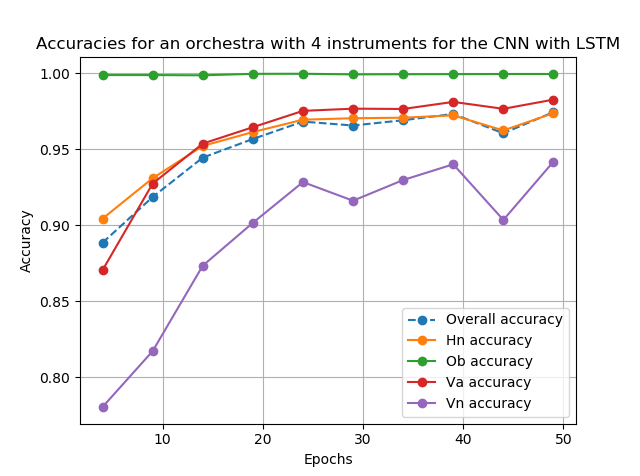
\includegraphics[scale=0.6]{figs/CNN4.png}
\end{figure}
\begin{figure}
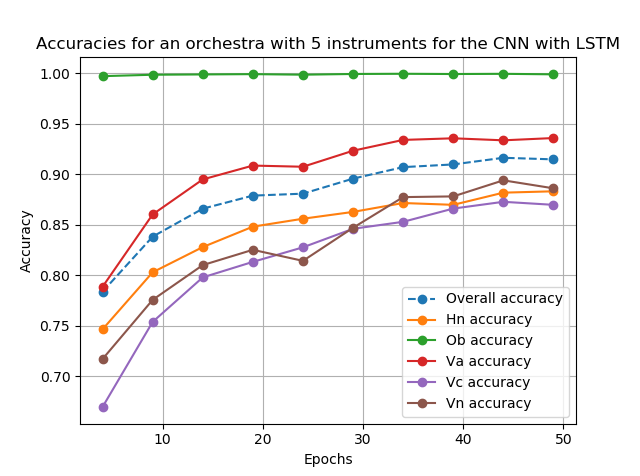
\includegraphics[scale=0.6]{figs/CNN5.png}
\end{figure}
\begin{figure}
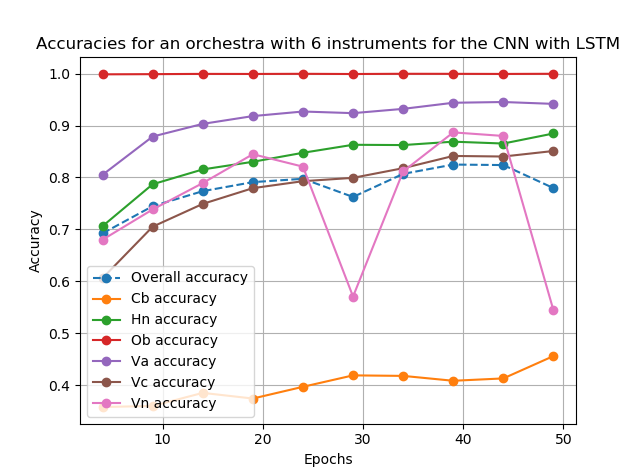
\includegraphics[scale=0.6]{figs/CNN6.png}
\end{figure}
\begin{figure}
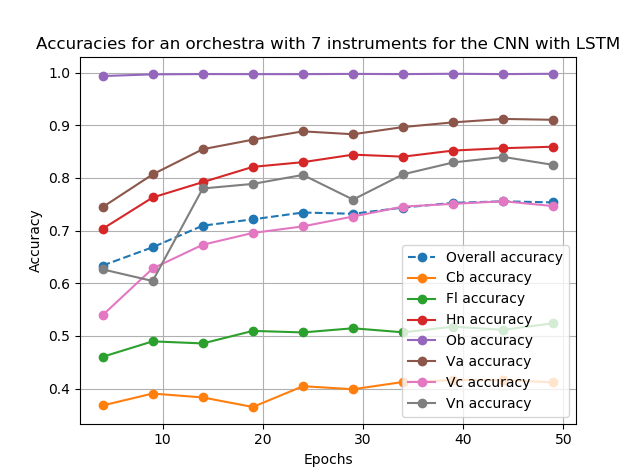
\includegraphics[scale=0.6]{figs/CNN7.png}
\end{figure}
\begin{figure}
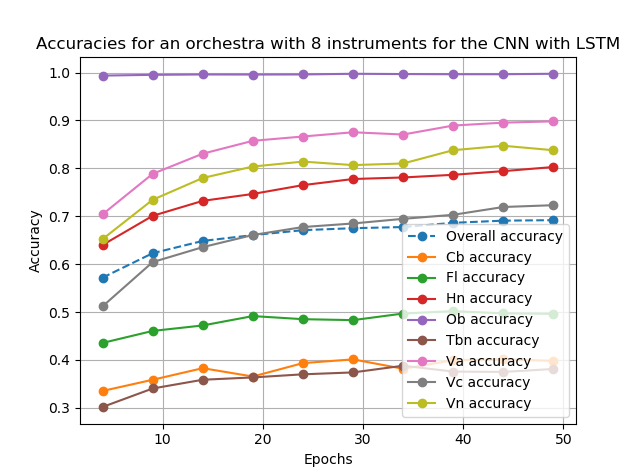
\includegraphics[scale=0.6]{figs/CNN8.png}
\end{figure}
\begin{figure}
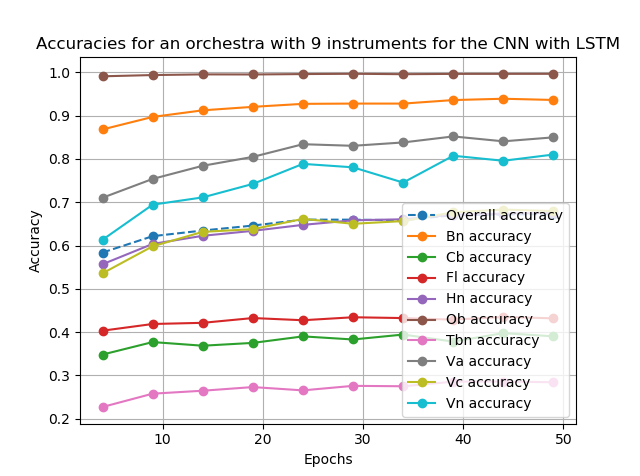
\includegraphics[scale=0.6]{figs/CNN9.png}
\end{figure}
\begin{figure}
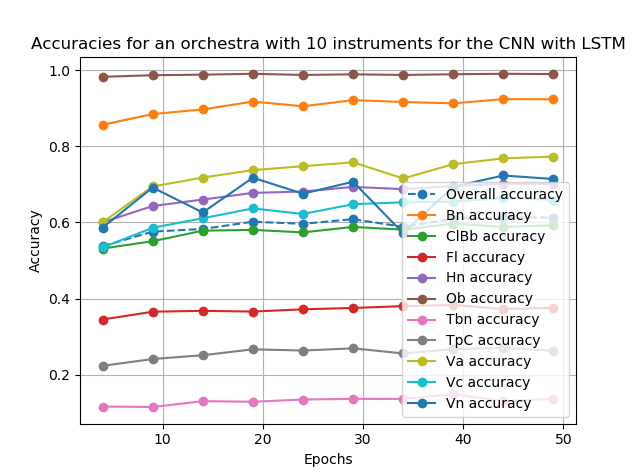
\includegraphics[scale=0.6]{figs/CNN10.png}
\end{figure}

% For bibtex users:
\bibliography{ISMIRtemplate}

% For non bibtex users:
%\begin{thebibliography}{citations}
%
%\bibitem {Author:00}
%E. Author.
%``The Title of the Conference Paper,''
%{\it Proceedings of the International Symposium
%on Music Information Retrieval}, pp.~000--111, 2000.
%
%\bibitem{Someone:10}
%A. Someone, B. Someone, and C. Someone.
%``The Title of the Journal Paper,''
%{\it Journal of New Music Research},
%Vol.~A, No.~B, pp.~111--222, 2010.
%
%\bibitem{Someone:04} X. Someone and Y. Someone. {\it Title of the Book},
%    Editorial Acme, Porto, 2012.
%
%\end{thebibliography}

\end{document}

